%\immediate\write18{tex ../tqft.dtx}
\documentclass{article}
\usepackage{tikz}
\usetikzlibrary{shapes.geometric,tqft}
\usepackage{tqft}

\tikzset{
  tqft/use nodes=false,
}

\begin{document}

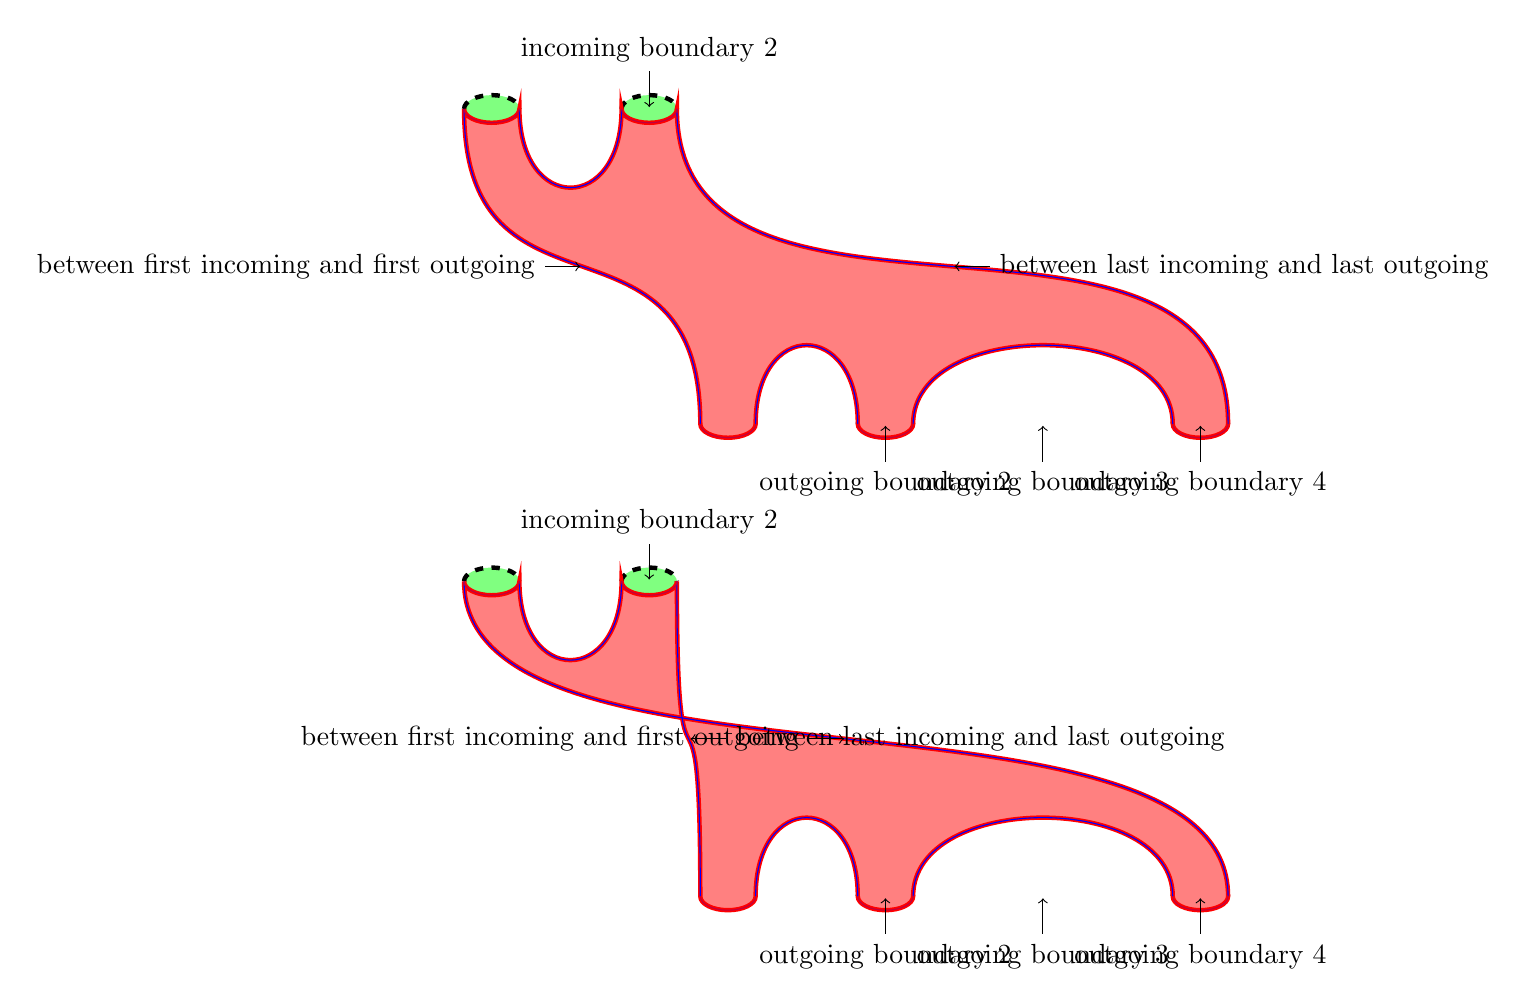
\begin{tikzpicture}[
  tqft,
  every outgoing boundary component/.style={fill=blue!50},
  outgoing boundary component 3/.style={fill=none,draw=red},
  every incoming boundary component/.style={fill=green!50},
  every lower boundary component/.style={draw,ultra thick, dashed},
  every upper boundary component/.style={draw,purple},
  cobordism/.style={fill=red!50,draw=red, ultra thick},
  cobordism edge/.style={draw,blue},
  view from=incoming,
  cobordism height=4cm,
  offset=1.5,
  incoming boundary components=2,
  outgoing boundary components=4,
  skip outgoing boundary components=3
]
\pic[
  name=a,
  tqft,
];
\pic[
  name=b,
  at={(0,-6)},
  tqft,
  twisted,
];

\begin{scope}[every pin edge/.style={<-}]
\foreach \cobordism in {a,b}
{
\foreach \anchor/\ang in {
%  hole 1/-90,
%  hole 2/90,
%  hole 3/-90,
  incoming boundary 2/90,
  outgoing boundary 2/-90,
  outgoing boundary 3/-90,
  outgoing boundary 4/-90,
  between last incoming and last outgoing/0,
  between first incoming and first outgoing/180%,
%  between incoming 1 and 3/90,
%  between outgoing 1 and 4/-90,
%  between outgoing 4 and 6/-90
} {
  \node[pin=\ang:\anchor,at=(\cobordism-\anchor),inner sep=0pt] {};
  }
  }
\end{scope}
\end{tikzpicture}


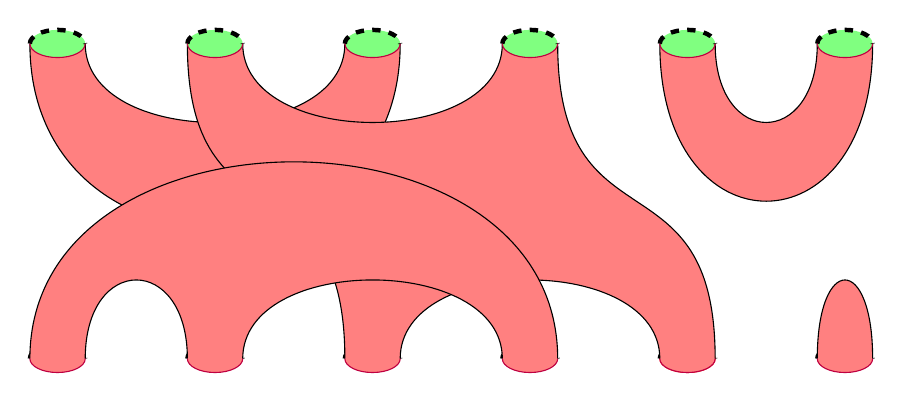
\begin{tikzpicture}[
  tqft,
  every outgoing boundary component/.style={fill=blue!50},
  outgoing boundary component 3/.style={fill=none,draw=red},
  every incoming boundary component/.style={fill=green!50},
  every lower boundary component/.style={draw,ultra thick, dashed},
  every upper boundary component/.style={draw,purple},
  cobordism/.style={fill=red!50},
  cobordism edge/.style={draw},
  view from=incoming,
  cobordism height=4cm,
]
\begin{scope}%[every node/.style={rotate=90}]
\pic[name=a,
  tqft,
  incoming boundary components=3,
  skip incoming boundary components=2,
  outgoing boundary components=0
  ];
\pic[name=b,
  tqft,
  incoming boundary components=3,
  skip incoming boundary components=2,
  outgoing boundary components=3,
  skip outgoing boundary components=2,
  offset=1,
  anchor=incoming boundary 1,
  at=(a-incoming boundary 2)
];
\pic[name=c,
  tqft,
  incoming boundary components=2,
  outgoing boundary components=0,
  anchor={(0,0)},
  at=(b-incoming boundary 3)
];
\pic[name=d,
  tqft,
  incoming boundary components=0,
  outgoing boundary components=4,
  skip outgoing boundary components=3,
  at=(a-incoming boundary 1)
];
\pic[name=e,
  tqft,
  incoming boundary components=0,
  outgoing boundary components=1,
  at=(c-incoming boundary 2)
];
\end{scope}
\end{tikzpicture}

%\end{document}
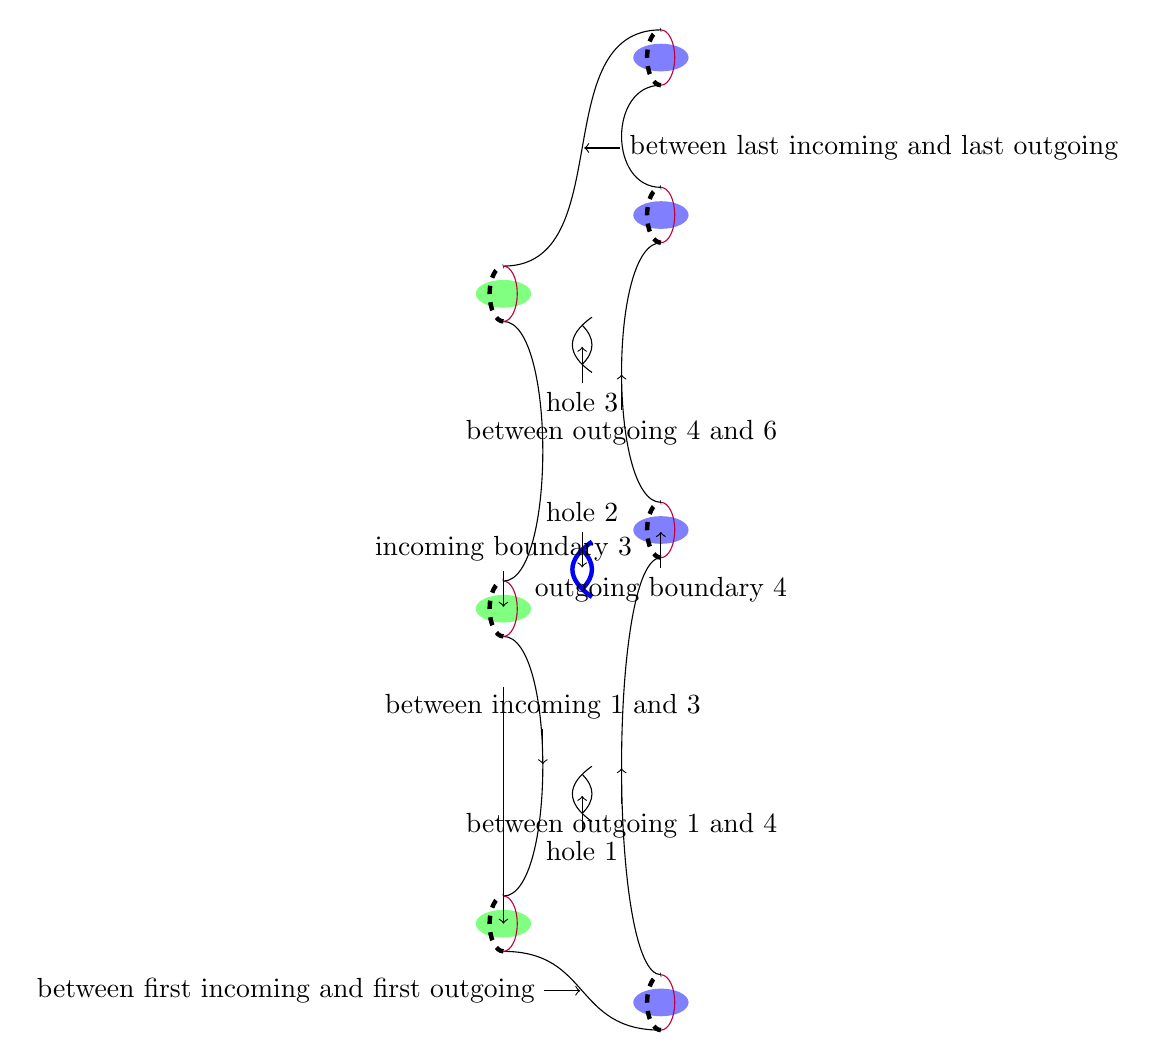
\begin{tikzpicture}[
  tqft,
  every outgoing boundary component/.style={fill=blue!50},
  outgoing boundary component 3/.style={fill=none,draw=red},
  every incoming boundary component/.style={fill=green!50},
  every lower boundary component/.style={draw,ultra thick, dashed},
  every upper boundary component/.style={draw,purple},
%  cobordism/.style={fill=red!50},
  cobordism edge/.style={draw},
  genus=3,
  hole 2/.style={ultra thick, blue},
  view from=incoming,
  anchor=between incoming 1 and 2
]
\begin{scope}[every node/.style={rotate=90}]
\pic[name=a,tqft,incoming boundary components=5,skip incoming boundary components={2,4},outgoing boundary components=7,skip outgoing boundary components={2,3,5},offset=-.5];
\end{scope}

\begin{scope}[every pin edge/.style={<-}]
\foreach \anchor/\ang in {
  hole 1/-90,
  hole 2/90,
  hole 3/-90,
  incoming boundary 3/90,
  outgoing boundary 4/-90,
  between last incoming and last outgoing/0,
  between first incoming and first outgoing/180,
  between incoming 1 and 3/90,
  between outgoing 1 and 4/-90,
  between outgoing 4 and 6/-90
} {
  \node[pin=\ang:\anchor,at=(a-\anchor),inner sep=0pt] {};
}
\draw[<-] (0,0) -- ++(0,3);
\end{scope}
\end{tikzpicture}
%\end{document}

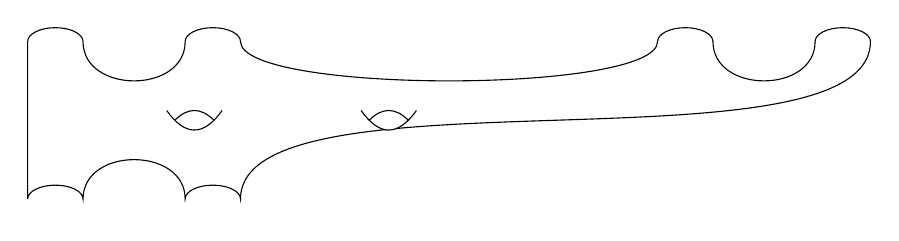
\begin{tikzpicture}
\pic[
  tqft,
  incoming boundary components=6,
  skip incoming boundary components={3,4},
  outgoing boundary components=2,
  genus=2,
  draw,
  name=a
];
\end{tikzpicture}
%\end{document}

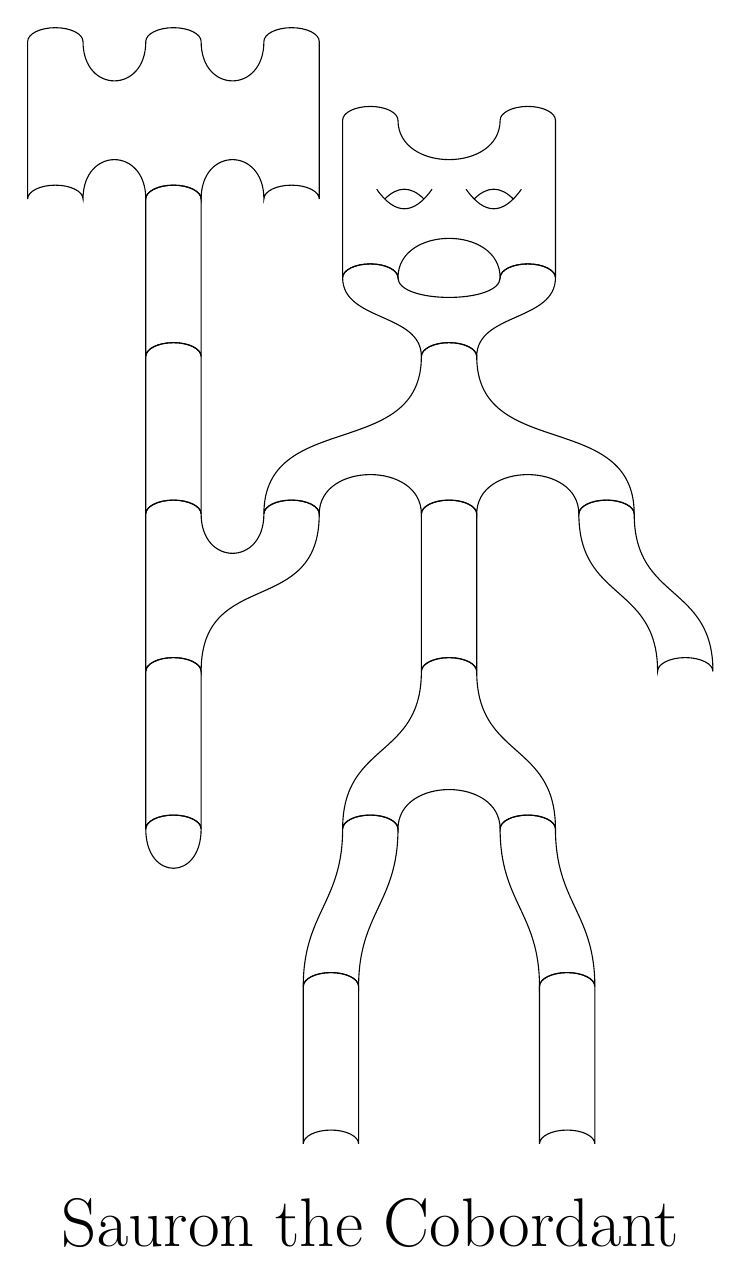
\begin{tikzpicture}
\pic[
  tqft,
  incoming boundary components=2,
  outgoing boundary components=2,
  genus=2,
  draw,
  name=a
];
\pic[
  tqft,
  incoming boundary components=2,
  outgoing boundary components=1,
  draw,
  at=(a-outgoing boundary 1),
  offset=.5,
  cobordism height=1cm,
  name=b
];
\pic[tqft,
  incoming boundary components=1,
  outgoing boundary components=3,
  draw,
  at=(b-outgoing boundary 1),
  offset=-1,
  name=c
];
\pic[tqft,
  incoming boundary components=2,
  outgoing boundary components=1,
  draw,
  at=(c-outgoing boundary 1),
  anchor=incoming boundary 2,
  name=d,
  boundary separation=1.5cm,
];
\pic[tqft,
  incoming boundary components=1,
  outgoing boundary components=1,
  draw,
  at=(c-outgoing boundary 3),
  offset=.5,
  name=e
];
\pic[tqft,
  incoming boundary components=1,
  outgoing boundary components=1,
  draw,
  at=(c-outgoing boundary 2),
  name=f
];
\pic[tqft,
  incoming boundary components=1,
  outgoing boundary components=2,
  draw,
  at=(f-outgoing boundary),
  name=g,
  offset=-.5,
];
\pic[tqft,
  incoming boundary components=1,
  outgoing boundary components=1,
  draw,
  at=(g-outgoing boundary 1),
  name=h,
  offset=-.25,
];
\pic[tqft,
  incoming boundary components=1,
  outgoing boundary components=1,
  draw,
  at=(g-outgoing boundary 2),
  name=i,
  offset=.25,
];
\pic[tqft,
  incoming boundary components=1,
  outgoing boundary components=1,
  draw,
  at=(h-outgoing boundary),
  name=j
];
\pic[tqft,
  incoming boundary components=1,
  outgoing boundary components=1,
  draw,
  at=(i-outgoing boundary),
  name=k
];
\pic[tqft,
  incoming boundary components=1,
  outgoing boundary components=1,
  draw,
  at=(d-outgoing boundary),
%  anchor={(1.5,0)},
  name=l
];
\pic[tqft,
  incoming boundary components=1,
  outgoing boundary components=0,
  draw,
  at=(l-outgoing boundary),
  name=m
];
\pic[tqft,
  incoming boundary components=1,
  outgoing boundary components=1,
  draw,
  at=(d-incoming boundary),
  anchor=outgoing boundary,
  name=n
];
\pic[tqft,
  incoming boundary components=1,
  outgoing boundary components=1,
  draw,
  at=(n-incoming boundary),
  anchor=outgoing boundary,
  name=o
];
\pic[tqft,
  incoming boundary components=3,
  outgoing boundary components=3,
  draw,
  at=(o-incoming boundary),
  anchor={(2,1)},
  name=p,
  boundary separation=1.5cm,
];
\path (j-outgoing boundary) ++(.5,-1) node {\Huge Sauron the Cobordant};
\end{tikzpicture}

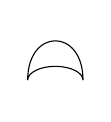
\begin{tikzpicture}
\pic[tqft cap,draw];
\end{tikzpicture}


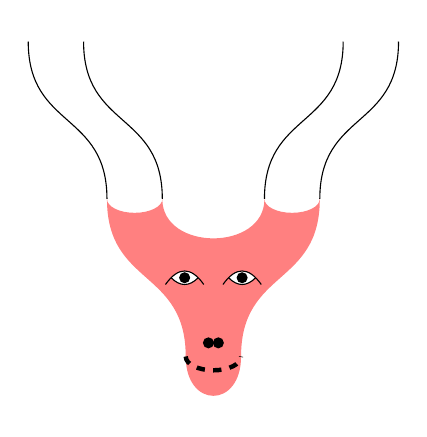
\begin{tikzpicture}
\pic[
  name=d,
  tqft cup,
  cobordism/.style={fill=red!50}];
\pic[
  name=a,
  tqft reverse pair of pants,
  genus=2,
  cobordism/.style={fill=red!50},
  genus style/.style={draw},
  view from=incoming,
  every outgoing upper boundary component/.style={draw, dashed, ultra thick},
  at=(d-incoming boundary),
  anchor=outgoing boundary
];
\pic[
  name=b,
  tqft cylinder to next,
  anchor=outgoing boundary 1,
  at=(a-incoming boundary),
  cobordism edge/.style={draw}
];
\pic[name=c,tqft cylinder to prior,anchor=outgoing boundary 1,cobordism edge/.style={draw},at=(a-incoming boundary 2)];
\fill (a-hole 1) circle[radius=2pt]  (a-hole 2) circle[radius=2pt];
\fill (a-outgoing boundary.70) circle[radius=2pt];
\fill (a-outgoing boundary.110) circle[radius=2pt];
\end{tikzpicture}


\begin{tikzpicture}[
  tqft,
  every outgoing boundary component/.style={fill=blue!50},
  outgoing boundary component 3/.style={fill=none,draw=red},
  every incoming boundary component/.style={fill=green!50},
  every lower boundary component/.style={draw,ultra thick, dashed},
  every upper boundary component/.style={draw,purple},
  cobordism/.style={fill=red!50},
  cobordism edge/.style={draw},
  genus=3,
  hole 2/.style={ultra thick, blue},
  view from=incoming,
  anchor=between incoming 1 and 2
]
\pic[name=a,tqft,incoming boundary components=2,outgoing boundary components=3,offset=-.5];
\begin{scope}[every pin edge/.style={<-}]
\foreach \anchor/\ang in {
  hole 1/-90,
  hole 2/90,
  hole 3/-90,
  incoming boundary 2/90,
  outgoing boundary 3/-90,
  between last incoming and last outgoing/0,
  between first incoming and first outgoing/180,
  between incoming 1 and 2/90,
  between outgoing 1 and 2/-90,
  between outgoing 2 and 3/-90
} {
  \node[pin=\ang:\anchor,at=(a-\anchor),inner sep=0pt] {};
}
\draw[<-] (0,0) -- ++(0,3);
\end{scope}
\end{tikzpicture}

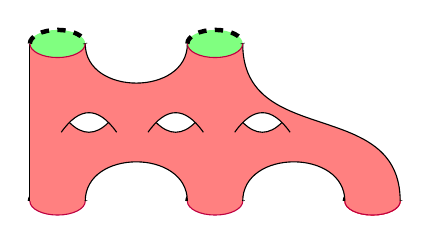
\begin{tikzpicture}[
  tqft,
  every outgoing boundary component/.style={fill=blue!50},
  outgoing boundary component 3/.style={fill=none,draw=red},
  every incoming boundary component/.style={fill=green!50},
  every lower boundary component/.style={draw,ultra thick, dashed},
  every upper boundary component/.style={draw,purple},
  cobordism/.style={fill=red!50},
  cobordism edge/.style={draw},
  genus=3,
  genus style/.style={draw},
  view from=incoming,
  anchor=between incoming 1 and 2
]
\pic[name=a,tqft,incoming boundary components=2,outgoing boundary components=3,offset=0];
\end{tikzpicture}

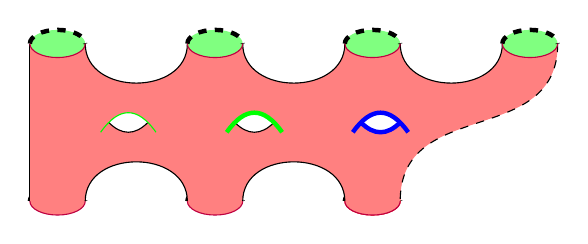
\begin{tikzpicture}[
  tqft,
  every outgoing boundary component/.style={fill=blue!50},
  outgoing boundary component 3/.style={fill=none,draw=red},
  every incoming boundary component/.style={fill=green!50},
  every lower boundary component/.style={draw,ultra thick, dashed},
  every upper boundary component/.style={draw,purple},
  cobordism/.style={fill=red!50},
  cobordism edge/.style={draw},
  genus=3,
  genus style/.style={draw},
  hole 3/.style={blue, ultra thick},
  genus upper/.style={green},
  hole 2 upper/.style={ultra thick},
  between last incoming and last outgoing/.style={dashed},
  view from=incoming,
  anchor=between incoming 1 and 2
]
\pic[name=a,tqft,incoming boundary components=4,outgoing boundary components=3,offset=0];
\end{tikzpicture}

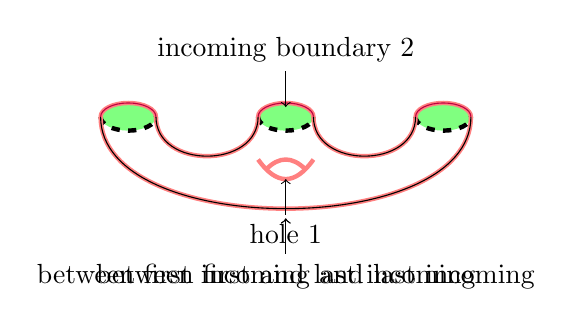
\begin{tikzpicture}[
  tqft,
  every outgoing boundary component/.style={fill=blue!50},
  outgoing boundary component 3/.style={fill=none,draw=red},
  every incoming boundary component/.style={fill=green!50},
  every lower boundary component/.style={draw,ultra thick, dashed},
  every upper boundary component/.style={draw,purple},
  cobordism/.style={draw=red!50,ultra thick},
  cobordism edge/.style={draw},
  genus=1
]
\pic[name=a,tqft,incoming boundary components=3,outgoing boundary components=0,offset=-.5];
\begin{scope}[every pin edge/.style={<-}]
\foreach \anchor/\ang in {
  hole 1/-90,
  incoming boundary 2/90,
  between first incoming and last incoming/-90,
  between first and last incoming/-90
} {
  \node[pin=\ang:\anchor,at=(a-\anchor)] {};
}
\end{scope}
\end{tikzpicture}


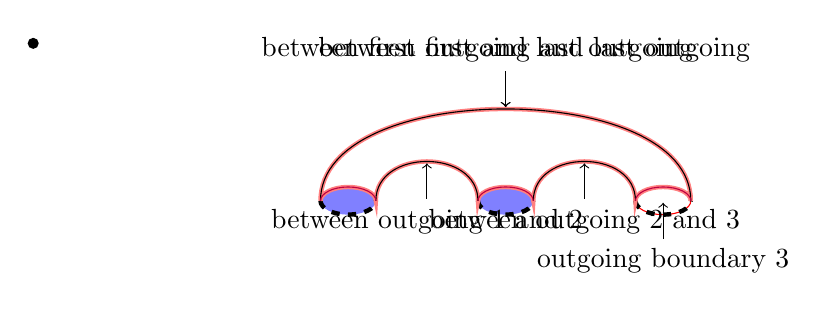
\begin{tikzpicture}[
  tqft,
  every outgoing boundary component/.style={fill=blue!50},
  outgoing boundary component 3/.style={fill=none,draw=red},
  every incoming boundary component/.style={fill=green!50},
  every lower boundary component/.style={draw,ultra thick, dashed},
  every upper boundary component/.style={draw,purple},
  cobordism/.style={draw=red!50,ultra thick},
  cobordism edge/.style={draw},
]
\pic[name=a,tqft,incoming boundary components=0,outgoing boundary components=3,offset=2];
\fill (0,0) circle[radius=2pt];
\begin{scope}[every pin edge/.style={<-}]
\foreach \anchor/\ang in {
  outgoing boundary 3/-90,
  between outgoing 1 and 2/-90,
  between outgoing 2 and 3/-90,
  between first and last outgoing/90,
  between first outgoing and last outgoing/90
} {
  \node[pin=\ang:\anchor,at=(a-\anchor),inner sep=0pt] {};
}
\end{scope}
\end{tikzpicture}


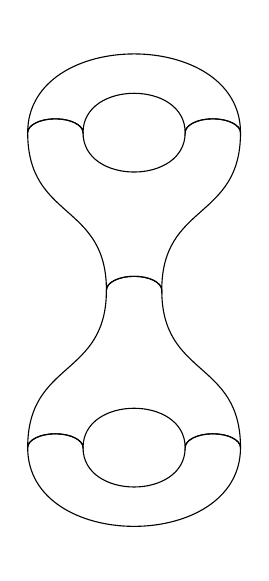
\begin{tikzpicture}[tqft/cobordism/.style={draw},every tqft/.style={transform shape},rotate=90,yscale=-1]
\pic[
  tqft,
  incoming boundary components=0,
  outgoing boundary components=2,
  name=a
];
\pic[
  tqft,
  incoming boundary components=2,
  outgoing boundary components=1,
  name=b,
  offset=.5,
  at=(a-outgoing boundary 1)
];
\pic[
  tqft,
  incoming boundary components=1,
  outgoing boundary components=2,
  offset=-.5,
  at=(b-outgoing boundary 1),
  name=c
];
\pic[
  tqft,
  incoming boundary components=2,
  outgoing boundary components=0,
  at=(c-outgoing boundary 1)
];
\end{tikzpicture}

\tikzset{tqft/use nodes=true}

\begin{tikzpicture}[tqft/flow=south]
\node[draw,tqft,incoming boundary components=2,outgoing boundary components=3,offset=-.5] (a) {};
\end{tikzpicture}

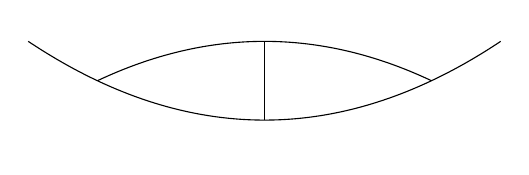
\begin{tikzpicture}
%\draw (0,0) .. controls +(2,4/3) and +(-2,4/3) .. (6,0);
\draw (0,1) .. controls +(2,-4/3) and +(-2,-4/3) .. (6,1);
\draw (3,0) -- (3,1);
\pgfmathsetmacro\xpos{(1 - 1/sqrt(2))/2}
\pgfmathsetmacro\sqrtwo{1/sqrt(2)}
\draw (6*\xpos,.5) .. controls +(2*\sqrtwo,2/3) and +(-2*\sqrtwo,2/3) .. (6 - 6*\xpos,.5);
\end{tikzpicture}


\begin{tikzpicture}[tqft/flow=east]
\node[tqft pair of pants, draw, boundary lower style={draw}] (a) {};
\node at (a.incoming boundary 1) {\(A\)};
\node at (a.outgoing boundary 1) {\(A\)};
\node at (a.outgoing boundary 2) {\(A\)};
\node at (a) {\(\beta\)};
\end{tikzpicture}


\begin{tikzpicture}[shape=tqft cobordism]
\begin{scope}[scale=2,rotate=45,tqft,flow=east,boundary lower style={draw,thick}]
\node[tqft pair of pants,draw,transform shape] {};
\end{scope}
\end{tikzpicture}
%\end{document}

\begin{tikzpicture}
\node[tqft pair of pants,draw,circle width=2cm,circle depth=1cm,cobordism height=8cm,boundary separation=2cm] {};
\end{tikzpicture}


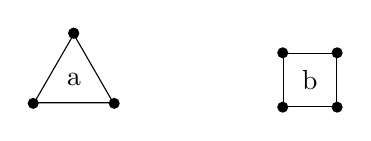
\begin{tikzpicture}
\node[regular polygon,regular polygon sides=3,draw] (a) {a};
\node[regular polygon,regular polygon sides=4,draw] (b) at (3,0) {b};
\foreach \k in {1,...,4} {
  \fill (a.corner \k) circle[radius=2pt];
}
\foreach \k in {1,...,4} {
  \fill (b.corner \k) circle[radius=2pt];
}
\end{tikzpicture}


\begin{tikzpicture}[tqft/flow={east}]
\fill[orange] (0,0) circle[radius=4pt];
\node[tqft,pair of pants,draw,outer sep=1cm] (a) at (0,0) {};
\node[tqft,incoming boundary components=4,outgoing boundary components=3,offset=.5,draw] (b) at (3,0) {};
%\node[tqft,pair of pants,draw,red] (b) at (1,0) {};
%\node[tqft,pair of pants,draw,green] (c) at (0,1) {};
%\node[tqft,pair of pants,draw,blue] (d) at (-1,0) {};
%\fill (a.incoming boundary 1) circle[radius=2pt];
%\fill[red] (b.incoming boundary 1) circle[radius=2pt];
%\fill[green] (c.incoming boundary 1) circle[radius=2pt];
%\fill[blue] (d.incoming boundary 1) circle[radius=2pt];
\foreach \anchor in {
  centre,
  center,
  north,
  south,
  east,
  north west,
  south west,
  north east,
  south east,
  west%
} {
\foreach \node/\colour in {
    a/black,
    b/red%,
%    c/green,
%    d/blue%
}{
\edef\command{\noexpand\fill[\colour] (\node.\anchor) circle[radius=2pt] node {\anchor};}
\command
}
}
\end{tikzpicture}


\begin{tikzpicture}
\node[draw,outer sep=1cm] (a) {a};
\fill (a.north) circle[radius=2pt];
\end{tikzpicture}

\begin{tikzpicture}[tqft/flow={east}]
\node[tqft,boundary circle,draw] at (0,0) {};
\node[tqft,boundary circle,draw,red] at (1,0) {};
\node[tqft,boundary circle,draw,green] at (0,1) {};
\node[tqft,boundary circle,draw,blue] at (-1,0) {};
\end{tikzpicture}

\begin{tikzpicture}[every tqft/.style={cobordism style={draw,thick,red}}]
 \node[
   tqft,
   fill=orange,
   fill opacity=.5,
   boundary style={fill=purple},
   cobordism style={draw,thick,red},
   boundary lower style={draw,dashed,thick,blue},
   boundary upper style={draw,green,thick},
   incoming boundary components=4,
   outgoing boundary components=6,
   offset=-1.5,
   outer sep=1cm,
 ] (a) {};
 \fill (a incoming 2.90) circle[radius=2pt];
 \fill (a outgoing 5.270) circle[radius=2pt];
 \fill (a incoming 2.centre) circle[radius=2pt];
 \fill (a outgoing 5.centre) circle[radius=2pt];
 \fill (a incoming 4.above) circle[radius=2pt];
 \fill (a outgoing 3.below) circle[radius=2pt];
 \fill (a.after incoming boundary 1) circle[radius=2pt] node[pin=north:between 1 and 2] {};
 \fill (a.after outgoing boundary 3) circle[radius=2pt] node[pin=south:between 3 and 4] {};
 \fill (a.incoming boundary 1) circle[radius=2pt] node[pin=north:1] {};
 \fill (a.incoming boundary 2) circle[radius=2pt] node[pin=north:2] {};
 \fill (a.incoming boundary 3) circle[radius=2pt] node[pin=north:3] {};
 \fill (a.incoming boundary 4) circle[radius=2pt] node[pin=north:4] {};
 \node[pin=north:2] at (a.incoming boundary 2) {};
 \node[pin=north:3] at (a.incoming boundary 3) {};
 \node[pin=north:4] at (a.incoming boundary 4) {};
 \node[pin=south:1] at (a.outgoing boundary 1) {};
 \node[pin=south:4] at (a.outgoing boundary 4) {};
 \node[pin=south:6] at (a.outgoing boundary 6) {};
\node[pin=west:west] at (a.west) {};
\node[pin=east:east] at (a.east) {};
 \end{tikzpicture}


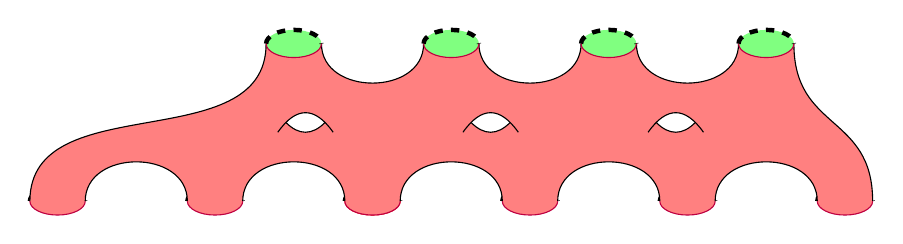
\begin{tikzpicture}[
  tqft/use nodes=false,
  tqft,
  every outgoing boundary component/.style={fill=blue!50},
  outgoing boundary component 3/.style={fill=none,draw=red},
  every incoming boundary component/.style={fill=green!50},
  every lower boundary component/.style={draw,ultra thick, dashed},
  every upper boundary component/.style={draw,purple},
  cobordism/.style={fill=red!50},
  cobordism edge/.style={draw},
  genus=3,
  genus style/.style={draw},
  view from=incoming,
  anchor=between incoming 1 and 2
]
\pic[name=a,tqft,incoming boundary components=4,outgoing boundary components=6,offset=-1.5];
\end{tikzpicture}



\begin{tikzpicture}[every tqft/.style={cobordism style={draw,thick,red}}]
 \node[
   tqft,
   fill=orange,
   fill opacity=.5,
   boundary style={fill=purple},
   cobordism style={draw,thick,red},
   boundary lower style={draw,dashed,thick,blue},
   boundary upper style={draw,green,thick},
   incoming boundary components=0,
   outgoing boundary components=6,
   offset=-1.5,
   outer sep=1cm,
 ] (aa) {hello world};
% \fill (aa incoming 2.90) circle[radius=2pt];
 \fill (aa outgoing 5.270) circle[radius=2pt];
% \fill (aa incoming 2.centre) circle[radius=2pt];
 \fill (aa outgoing 5.centre) circle[radius=2pt];
% \fill (aa incoming 4.above) circle[radius=2pt];
 \fill (aa outgoing 3.below) circle[radius=2pt];
 \fill (aa.incoming boundary 1) circle[radius=2pt] node[pin=north:1] {};
 \fill (aa.incoming boundary 2) circle[radius=2pt] node[pin=north:2] {};
 \fill (aa.incoming boundary 3) circle[radius=2pt] node[pin=north:3] {};
 \fill (aa.incoming boundary 4) circle[radius=2pt] node[pin=north:4] {};
 \node[pin=north:2] at (aa.incoming boundary 2) {};
 \node[pin=north:3] at (aa.incoming boundary 3) {};
 \node[pin=north:4] at (aa.incoming boundary 4) {};
 \node[pin=south:1] at (aa.outgoing boundary 1) {};
 \node[pin=south:4] at (aa.outgoing boundary 4) {};
 \node[pin=south:6] at (aa.outgoing boundary 6) {};
\fill[cyan] (0,0) circle[radius=3pt];
\node[pin=west:west] at (aa.west) {};
\node[pin=east:east] at (aa.east) {};
\node[pin=north:north] at (aa.north) {};
 \end{tikzpicture}

\begin{tikzpicture}[tqft/flow={east},every tqft/.style={cobordism style={draw,thick,red}}]
 \node[
   tqft,
   boundary circle,
   circle width=2cm,
   circle depth=1cm,
   boundary separation=4cm,
   fill=orange,
   fill opacity=.5,
   boundary style={fill=purple},
   cobordism style={draw,thick,red},
   boundary lower style={draw,dashed,thick,blue},
   boundary upper style={draw,green,thick},
   incoming boundary components=4,
   outgoing boundary components=6,
   offset=-1.5,
 ] (a) {};
 \node[
   tqft,
   boundary circle,
   circle width=2cm,
   circle depth=1cm,
   boundary separation=4cm,
   fill=orange,
   fill opacity=.5,
   boundary style={fill=purple},
   cobordism style={draw,thick,red},
   boundary lower style={draw,dashed,thick,blue},
   boundary upper style={draw,green,thick},
   incoming boundary components=4,
   outgoing boundary components=6,
   offset=-1.5,
 ] at (5,0) (b) {hello world};
\fill[red] (b.centre) circle[radius=2pt];
 \fill[red] (b.next) circle[radius=2pt] node[pin=north:next] {};
 \fill[red] (b.prior) circle[radius=2pt] node[pin=north:prior] {};
 \fill[red] (b.above) circle[radius=2pt] node[pin=north:above] {};
 \fill[red] (b.below) circle[radius=2pt] node[pin=north:below] {};
 \fill (a.next) circle[radius=2pt] node[pin=north:next] {};
 \fill (a.prior) circle[radius=2pt] node[pin=north:prior] {};
 \fill (a.above) circle[radius=2pt] node[pin=north:above] {};
 \fill (a.below) circle[radius=2pt] node[pin=north:below] {};
 \draw (0,0) -- (90:2);
 \draw (0,0) -- (0:2);
 \draw (0,0) -- (180:2);
 \draw (0,0) -- (270:2);
\foreach \ang in {0,20,...,340} {
 \fill (a.\ang) circle[radius=2pt] node[pin=\ang:\ang] {};
 \draw (0,0) -- (\ang:2);
}
 \end{tikzpicture}

\end{document}

% Local Variables:
% tex-output-type: "pdf18"
% End:
